\documentclass{beamer}

\usefonttheme{serif}

\usepackage{graphicx}
\usepackage{xcolor}
\usepackage{colortbl}
\usepackage{multirow,tabularx}
\usepackage{tikz}
\usepackage{hyperref}

\usetikzlibrary{positioning, arrows.meta}

\hypersetup{
    colorlinks=true,
    linkcolor=blue,
    urlcolor=blue
}

%------------------------------------------------

\title{\textcolor{blue}{Introduction to Image Processing}}
\subtitle{\textcolor{blue}{Wigner Summer Camp\\
Data and Compute Intensive Sciences Research Group}}

\author{
\textcolor{blue}{
Balázs, Paszkál, Vince, Levente, Bence, Antal\\
Éva, Hajni
}
}

\date{\textcolor{blue}{6--10 July 2026}}


%------------------------------------------------
% Footer

\setbeamertemplate{footline}{
\leavevmode%
\hbox{
\begin{beamercolorbox}
[wd=.1\paperwidth,ht=2.25ex,dp=1ex,left]
{page number in head/foot}

\hspace{1em}
\textcolor{blue}{\insertframenumber}

\end{beamercolorbox}
}
\vskip0pt
}


%------------------------------------------------
% Section slides

\AtBeginSection{
\begin{frame}{Outline}
    \tableofcontents[currentsection]
\end{frame}
}


%================================================

\begin{document}


% Title

\begin{frame}

    \titlepage

    \vspace{-0.5cm}

    \centering
    
\includegraphics[width=0.25\textwidth]{../img/logo.png}

\end{frame}


%================================================


\section{Introduction}


\begin{frame}{Project Overview}

    \begin{itemize}

        \item Image processing techniques for extracting useful information

        \item Filtering, transformations and feature extraction

        \item Python based implementation

        \item Goal: analyze and enhance digital images

    \end{itemize}

\end{frame}


%------------------------------------------------


\begin{frame}{What is Image Processing?}

    \begin{block}{Definition}

        Image processing is the manipulation and analysis of digital images
        to improve quality or extract important information.

    \end{block}


    \begin{itemize}

        \item Image enhancement

        \item Noise reduction

        \item Edge detection

        \item Feature extraction

    \end{itemize}

\end{frame}



%================================================

\section{Pipeline}


\begin{frame}{Main Pipeline}

    \centering


    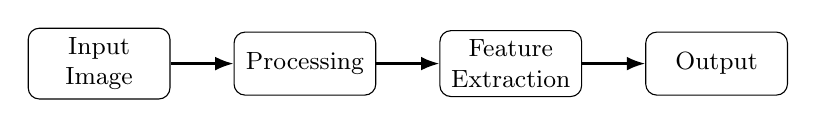
\begin{tikzpicture}[
            box/.style={
                    draw,
                    rounded corners,
                    minimum width=1.8cm,
                    minimum height=0.8cm,
                    align=center,
                    font=\small
                },
            arrow/.style={
                    -{Latex},
                    thick
                }
        ]


        \node[box] (input)
        {Input\\Image};


        \node[box,right=0.8cm of input]
        (process)
        {Processing};


        \node[box,right=0.8cm of process]
        (feature)
        {Feature\\Extraction};


        \node[box,right=0.8cm of feature]
        (output)
        {Output};


        \draw[arrow](input)--(process);
        \draw[arrow](process)--(feature);
        \draw[arrow](feature)--(output);


    \end{tikzpicture}


\end{frame}



%------------------------------------------------


\begin{frame}{Architecture}

    \centering


    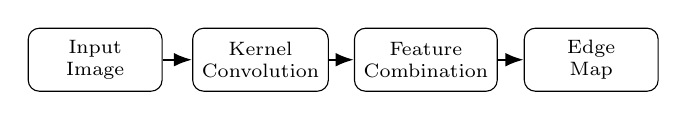
\begin{tikzpicture}[
            box/.style={
                    draw,
                    rounded corners,
                    minimum width=1.7cm,
                    minimum height=0.8cm,
                    align=center,
                    font=\scriptsize
                },
            arrow/.style={
                    -{Latex},
                    thick
                }
        ]


        \node[box] (img) at (0,0)
        {Input\\Image};


        \node[box] (conv) at (2.1,0)
        {Kernel\\Convolution};


        \node[box] (comb) at (4.2,0)
        {Feature\\Combination};


        \node[box] (out) at (6.3,0)
        {Edge\\Map};


        \draw[arrow](img)--(conv);
        \draw[arrow](conv)--(comb);
        \draw[arrow](comb)--(out);


    \end{tikzpicture}


    \vspace{0.4cm}


    \begin{itemize}

        \item Image passes through convolution operations

        \item Features are extracted

        \item Output represents important structures


    \end{itemize}


\end{frame}



%================================================


\section{Methods}



\begin{frame}{Core Methods}


    \begin{columns}


        \column{0.5\textwidth}

        \textbf{Filtering}

        \begin{itemize}

            \item Blur

            \item Sharpening

            \item Noise removal

        \end{itemize}



        \column{0.5\textwidth}

        \textbf{Detection}

        \begin{itemize}

            \item Edge detection

            \item Feature extraction

            \item Image analysis

        \end{itemize}


    \end{columns}


\end{frame}



%------------------------------------------------


\begin{frame}{Technology Stack}


    \begin{tabular}{ll}

        Language  & Python                    \\

        Libraries & OpenCV, NumPy, Matplotlib \\

        Input     & Digital images            \\

        Output    & Processed images          \\
    \end{tabular}


\end{frame}



%================================================


\section{Applications}



\begin{frame}{Applications}


    \begin{itemize}

        \item Computer vision systems

        \item Object detection

        \item Medical image analysis

        \item Autonomous systems

        \item Industrial inspection


    \end{itemize}


\end{frame}



%------------------------------------------------


\begin{frame}{Summary}


    \begin{block}{Conclusion}

        Image processing allows computers to analyze and manipulate
        visual information using mathematical methods.

    \end{block}


    \begin{itemize}

        \item Transform images

        \item Extract features

        \item Detect patterns


    \end{itemize}


\end{frame}



%------------------------------------------------




\end{document}